% Geombinatorics format: 8.5in x 5.5in (landscape half-letter), margins 0.35in top/left/right and 0.5in bottom,
% Times 11pt single-spaced, title in bold capitals 14pt, no page numbers.
\documentclass[11pt]{article}
\usepackage[paperwidth=8.5in,paperheight=5.5in,top=0.35in,left=0.35in,right=0.35in,bottom=0.5in,includefoot=false]{geometry}
\usepackage{mathptmx}
\usepackage{graphicx,booktabs,amsmath,amsthm}
\usepackage[hidelinks]{hyperref}
\pagestyle{empty}
\setlength{\parskip}{3pt}
\newtheorem*{theorem}{Theorem}
\begin{document}
\thispagestyle{empty}
\begin{center}
{\fontsize{14}{17}\selectfont\bfseries TWELVE UNIT CUBES IN A CUBE OF SIDE 2.93152}\\[6pt]
Yohei Nakajima\\
{\small yohei@untapped.vc}
\end{center}

\begin{abstract}\noindent
We give a packing of 12 non-overlapping unit cubes in a cube of side $2.9315185094797$, with every pair of cubes and every wall at least $10^{-6}$ apart. The previous best known side was $2.9327717687\ldots$ (H.~Lin, July 2026). The packing was found by compressing unit-diameter balls in a shrinking box and hardening them into cubes under continued inward pressure. Coordinates, a short verifier and an exact certificate are public.
\end{abstract}

\section*{1. The problem}
Let $s(n)$ be the side of the smallest cube that contains $n$ non-overlapping unit cubes, which may be rotated. The known values are few. Friedman's catalogue \cite{friedman} lists non-trivial packings only for $n=9$--$14$ and $28$--$33$; for every other $n<34$ the trivial packing in a $\lceil n^{1/3}\rceil$-cube is the best known. From 1998 the best known side for $n=12$ was $2+2\sqrt2/3\approx2.94281$ (Friedman); in July 2026 H.~Lin improved it to $2.93277177\ldots$, with coordinates published in \cite{hyra}.

\begin{theorem}
Twelve unit cubes fit in a cube of side $2.9315185094797$. Hence $s(12)\le 2.93152$.
\end{theorem}

\section*{2. The packing}
Table~1 lists the twelve cubes. Cube $i$ is the unit cube $c_i + R(q_i)\,[-\tfrac12,\tfrac12]^3$, where $c_i$ is its centre and $R(q_i)$ the rotation given by the unit quaternion $q_i=(w,x,y,z)$; the container is $[0,s]^3$ with $s=2.9315185094797$. Four cubes are exactly axis-parallel, two are tilted by less than $1^\circ$, and six are tilted by $9^\circ$ or more (Figure~1). Full-precision values are in the file \texttt{cubincub\_n12.json} \cite{repo}.

\begin{center}\scriptsize
\begin{tabular}{rrrrrrrr}\toprule
$i$ & $x$ & $y$ & $z$ & $w$ & $q_x$ & $q_y$ & $q_z$\\\midrule
1 & 1.5243900087 & 2.4315173049 & 1.3320181026 & 0.5838886869 & -0.5838886869 & -0.3988408220 & -0.3988408220 \\
2 & 2.4315175095 & 2.4315173049 & 0.5000010000 & 0.7071067812 & 0.7071067812 & -0.0000000000 & 0.0000000000 \\
3 & 0.5000010000 & 1.4369556928 & 1.4377218077 & 0.5395289954 & 0.4570650535 & 0.4570650535 & -0.5395289954 \\
4 & 0.5098745912 & 0.5769319953 & 2.3545775829 & 0.4560511351 & -0.5403863020 & -0.4560472394 & 0.5403896022 \\
5 & 0.6086104699 & 2.2929309153 & 2.3887769910 & 0.0258332833 & 0.7609821302 & -0.6482073268 & -0.0081302199 \\
6 & 2.4315175095 & 1.4315163049 & 0.5000010000 & 0.0000000000 & -0.0000000000 & -0.0000000000 & -1.0000000000 \\
7 & 2.4298431049 & 2.4215276465 & 2.2620542416 & 0.0000269579 & 0.0016621483 & -0.9999712786 & 0.0073944948 \\
8 & 1.5800409188 & 1.4806927085 & 2.4315175095 & 0.0000000000 & -0.9765112947 & -0.2154662186 & -0.0000000000 \\
9 & 1.6870691741 & 0.7046058868 & 1.3931640729 & 0.1630483719 & -0.8266039691 & -0.3023204668 & 0.4458065074 \\
10 & 0.6714203714 & 0.5125513149 & 0.5042794969 & 0.0019279356 & 0.0017767559 & -0.7100527881 & -0.7041435680 \\
11 & 2.4315175095 & 0.5648571561 & 2.4315175095 & 0.5000000000 & -0.5000000000 & -0.5000000000 & 0.5000000000 \\
12 & 0.5000010000 & 2.3777515563 & 0.5000010000 & 0.7071067812 & -0.7071067812 & 0.0000000000 & 0.0000000000 \\
\bottomrule
\end{tabular}\\[2pt]
{\small Table 1. Centres and rotation quaternions, rounded to 10 decimals.}
\end{center}

\begin{center}
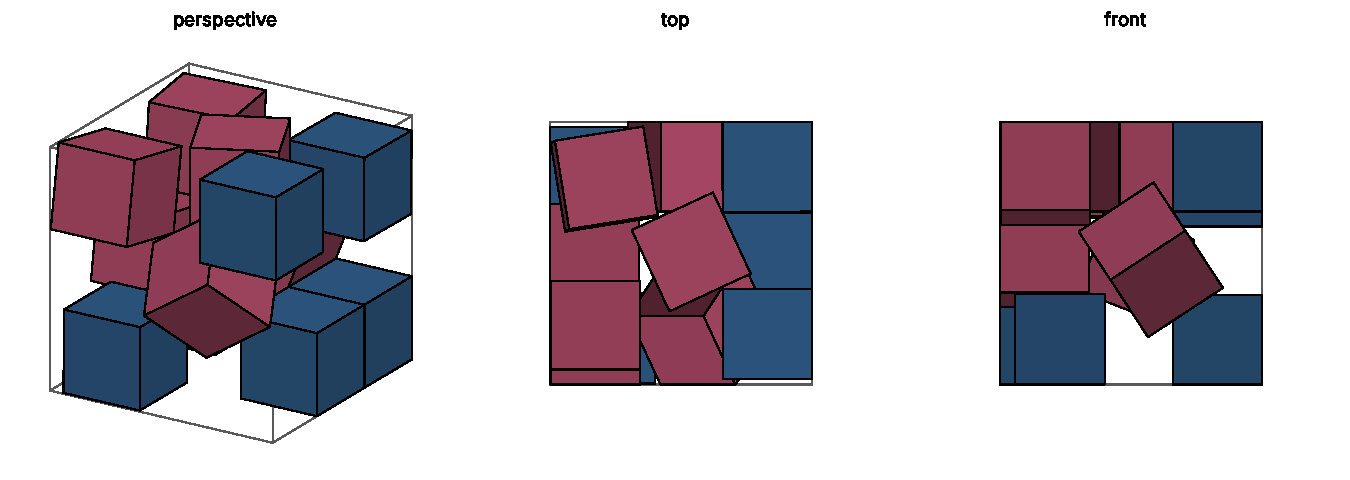
\includegraphics[height=2.3in]{../figures/n12_views.pdf}\\[-2pt]
{\small Figure 1. The packing from three directions. Red cubes are tilted.}
\end{center}

\section*{3. Verification}
For each cube, rotate the eight corners $(\pm\frac12,\pm\frac12,\pm\frac12)$ by $q_i$ and translate by $c_i$. All corners lie in $[0,s]^3$; the smallest distance from a corner to a wall is $1.000000000\cdot10^{-6}$. Two boxes are disjoint if and only if one of fifteen axes separates their projections: the three face normals of each cube and the nine cross products of their edge directions. Over all 66 pairs the smallest separation along such an axis is $1.000000001\cdot10^{-6}$. A 30-line program that performs these checks, \texttt{verify.py}, is in \cite{repo}.

The same checks were repeated in exact rational arithmetic. Every number in the file was converted to a rational, each rotation was taken as $H(q)/|q|^2$ (exactly orthogonal for any $q\ne0$, where $H$ is the homogeneous quaternion matrix), every corner was confirmed to lie in $[0,s]^3$, and for each pair an explicit rational plane was exhibited that strictly separates the two cubes. The program is \texttt{certify\_exact.py} in \cite{repo}.

\section*{4. How it was found}
Each cube begins as a ball of diameter 1 and is replaced, over the course of the search, by the \emph{rounded cube} of softness $r$: a cube of half-side $\frac12-r$ enlarged by a ball of radius $r$. At $r=\frac12$ this is the ball, at $r=0$ the unit cube, and every intermediate shape lies inside the unit cube. Starting from random positions, the balls are compressed under inward pressure on the container; then $r$ is lowered to $0$ while the pressure continues, so the shapes grow into cubes as the box settles around them. Overlaps are penalized and positions, orientations and the box size follow gradient descent. The best configuration was then tightened by a constrained optimizer that keeps every corner inside the box and a separating plane between every nearby pair, and finally spread by a factor $1+10^{-6}$ to give the stated clearance.

Two of 192 random starts landed below the previous record, in two different arrangements ($2.931515$ and $2.931620$ before clearance was added). The same procedure started with rigid cubes did not come within $0.05$ of the record. On squares in a square, the method recovers the best known packings for $n=11$, $17$, $18$, $19$, $26$ and $27$ from random starts \cite{repo}.

\section*{5. Remarks}
Several quaternions in Table~1 have repeated components, which suggests a closed form for the side. We have not found it. We use no lower bound beyond the volume bound $s(12)\ge 12^{1/3}\approx2.289$; how close $2.93152$ is to optimal is open. For $n=11$ the same search reached $2+2/\sqrt5\approx2.894427$, above Lin's $2.88295$; for $n=13$ and $14$ it did not improve the catalogue.

\section*{Acknowledgement}
Code, experiments and verification were developed with Claude (Anthropic), an AI system, under the author's direction. The author takes responsibility for the content.

\begin{thebibliography}{9}\small
\bibitem{friedman} E.~Friedman, \emph{Cubes in Cubes}, Erich's Packing Center, \url{https://erich-friedman.github.io/packing/cubincub/} (accessed 8 October 2026).
\bibitem{hyra} Tencent Hunyuan, \emph{Hyra-results: packing records}, file \texttt{cubincub\_n12.json}, \url{https://github.com/Tencent-Hunyuan/Hyra-results} (accessed 8 October 2026).
\bibitem{repo} Y.~Nakajima, \emph{soft-to-rigid-packing}, version 1.0.0, \url{https://github.com/yoheinakajima/soft-to-rigid-packing} (2026).
\end{thebibliography}
\end{document}
